		
		\documentclass[fleqn]{tukseminar}
		
		% Specify that the source file has UTF8 encoding
		\usepackage[utf8]{inputenc}
		% Set up the document font; font encoding (here T1) has to fit the used font.
		\usepackage[T1]{fontenc}
		\usepackage{lmodern}
		
		% Load language spec
		\usepackage[english]{babel}
		% German article --> ngerman (n for »neue deutsche Rechtschreibung«)
		% British English --> english
		
		% Ffor bibliography and \cite
		\usepackage{cite}
		
		% AMS extensions for math typesetting
		\usepackage[intlimits]{mathtools}
		\usepackage{amssymb}
		% ... there are many more ...
		\usepackage{multicol}
		% Fixes some unpleasantries in the kernel that have not yet adapted upstream
		% May be obsolete if you have a current installation.
		\usepackage{fixltx2e}
		
		% Load \todo command for notes
		\usepackage{todonotes}
		
		% Sebastian's favorite command for large inline todonotes
		% Caveat: does not work well with \listoftodos
		\newcommand\todoin[2][]{\todo[inline, caption={2do}, #1]{
				\begin{minipage}{\linewidth-1em}\noindent\relax#2\end{minipage}}}
		
		% Load \includegraphics command for including pictures (pdf or png highly recommended)
		\usepackage{graphicx}
		
		% Typeset source/pseudo code
		\usepackage{listings}
		
		% Load TikZ library for creating graphics
		% Using the PGF/TikZ manual and/or tex.stackexchange.com is highly adviced.
		\usepackage{tikz}
		% Load tikz libraries needed below (see the manual for a full list)
		\usetikzlibrary{automata,positioning}
		
		\usetikzlibrary{shapes,arrows,shadows}
		
		% Load \url command for easier hyperlinks without special link text
		\usepackage{url}
		
		% Load support for links in pdfs
		\usepackage{hyperref}
		
		% Use inconsolata font for code:
		\usepackage{inconsolata}
		
		
		%TLA+Typesetting
		\usepackage{tlaTypesetting}
		
		%Graph visualization
		\usepackage{pdfpages}
		\usepackage{float}
		\usepackage{longtable}
		
		
		% Defines default styling for code listings
		\definecolor{gray_ulisses}{gray}{0.55}
		\definecolor{green_ulises}{rgb}{0.2,0.75,0}
		\lstset{%
			columns=flexible,
			keepspaces=true,
			tabsize=3,
			basicstyle={\fontfamily{tx}\ttfamily\small},
			stringstyle=\color{green_ulises},
			commentstyle=\color{gray_ulisses},
			identifierstyle=\slshape{},
			keywordstyle=\bfseries,
			numberstyle=\small\color{gray_ulisses},
			numberblanklines=false,
			inputencoding={utf8},
			belowskip=-1mm,
			escapeinside={//*}{\^^M} % Allow to set labels and the like in comments
		}
		
		% Defines a custom environment for indented shell commands
		\newenvironment{displayshellcommand}{%
			\begin{quote}%
				\ttfamily%
			}{%
			\end{quote}%
		}
		
		%%%%%%%%%%%%%%%%%%%%%%%%%%%%%%%%%%%%%%%%%%%%%%%%%%%%%%%%%%%%%%%%%%%%%%%%%%%%%%%
		
		\title{Seminar "Verification and Model checking"}
		\event{Seminar: Software Engineering in Winter term 2020}
		\author{Ayush Pandey
			\institute{Technische Universität Kaiserslautern, Department of Computer Science}}
		
		%%%%%%%%%%%%%%%%%%%%%%%%%%%%%%%%%%%%%%%%%%%%%%%%%%%%%%%%%%%%%%%%%%%%%%%%%%%%%%%
		\begin{document}
			%%%%%%%%%%%%%%%%%%%%%%%%%%%%%%%%%%%%%%%%%%%%%%%%%%%%%%%%%%%%%%%%%%%%%%%%%%%%%%%
			
			\maketitle
			
			%%%%%%%%%%%%%%%%%%%%%%%%%%%%%%%%%%%%%%%%%%%%%%%%%%%%%%%%%%%%%%%%%%%%%%%%%%%%%%%
			
			\begin{abstract}
				
			\end{abstract}
			
			%%%%%%%%%%%%%%%%%%%%%%%%%%%%%%%%%%%%%%%%%%%%%%%%%%%%%%%%%%%%%%%%%%%%%%%%%%%%%%
			
			\section{Abstract}
			\label{sec:introduction}
			Modern information systems are growing in size, both, in terms of the number of components they are constructed from and the individual complexities of the components themselves. A single processor in a modern day personal computer has the capability of executing millions of instructions per second. The task of harnessing the power of these systems, however, comes with a challenge.
			
			With the systems size increasing, the code base for software systems very often reaches millions of lines of code. It is therefore inevitable that some errors are present in the systems. Exhaustive testing of the functionalities is one way to ascertain the correctness, but it is also time-consuming and requires a significant amount of effort to cover all critical and edge cases.
			
			Software systems implement a solution to a real world problem. Hence, it is possible to formally model them. The most common way of modelling systems is through labelled transition diagrams, also called state machines. These transition diagrams can be further represented as logical formulas with varying degrees of detail. With a successful model of the system, Model checking provides a way to formally check if this model meets the requirements of a given specification.
			
			The problem we ta\label{key}ckled in this seminar is a classical algorithm in the distributed and concurrent algorithms. Mutual exclusion\cite{wiki:mutex} is a property which specifies concurrency control for the purpose of preventing race conditions over accesses to a shared resource. The requirement is that in a concurrent setting where multiple processes (or threads) use the same resource, a process never enters a critical section while another process is entering or is already in its critical section. One of the ways to introduce mutual exclusion in a system is to use locks. A classical example of a lock is \textbf{Peterson's Algorithm} or Peterson's Lock.
			
			There are several tools which have been developed to automate and simplify the process of model checking. Some examples are: \tla, BLAST\cite{blast}, Java Pathfinder\cite{pathfinder}, Promela\cite{promela}, Isabelle\cite{isabelle} etc. In this report, we discuss the two major methods of software verification, namely, \textbf{Model checking} and \textbf{Deduction}. We also present the differences between the two approaches and how software verification can be done using \tla
			
			\newpage
			
			
			\tableofcontents
			
			\newpage
			
			\section{Introduction to Software Verification}
			Software verification aims towards checking whether the specified system fulfils the qualitative requirements that have been identified. Such verification is typically done using formal methods of mathematics. 
			
			There are two major approaches that can be taken to perform software verification, \textbf{Model checking} and \textbf{Deduction}. With model checking, a systematic exhaustive exploration of the states of the system is performed. This is usually only possible if the system follows a finite behavioural model or where the states can be represented finitely by abstraction. While model checking is often fully automatic, it does not perform well with systems which are significantly large. 
			
			The deductive approach deals with \textit{proof obligations} and is also referred to as \textit{Theorem proving}. The interpretation of the obligation decides the conformance of the system with the property being verified. Generally, the obligations are checked against the specification of the system using proof assistants. \tlaps is the proof assistant that \tla uses. Theorem proving is an involved process. It requires the user to know both, the mathematical foundation of the system, as well as, how the correctness can be specified using the constructs of the proof language. In this report, we present in detail how a proof is written in \tla.
			
			\section{The\tla Language}
			\label{sec:tlalanguage}
			
			\subsection{Introduction}
			\tla is a formal specification language. TLA is an acronym for \textbf{Temporal Logic of Actions}\cite{DBLP:journals/toplas/Lamport94}. It was developed by Leslie Lamport in 1999. The main use of \tla is towards specifying concurrent and distributed systems. The models in \tla follow a mathematical approach and are based on \textbf{First-order logic }and \textbf{Zermelo-Fraenkel set theory}. The purpose of employing a formal verification tool is to identify the flaws in the system before the model is realized in any programming language and a concrete implementation is undertaken. In \tla, the models are referred to as \textbf{specifications}. The term specification is used henceforth in this document.
			
			\tla has an IDE which is used for specifying systems, performing the model checking and proving theorems. Of the two, the model checker has a more widespread and common use case. 
			
			\subsection{Specifying a system in \tla}
			
			Consider as an example, the specification of a bank. Such a system requires account holders and transactions. Account-holders, each, have a certain amount of money, we call it \textbf{balance} and a transaction is used to transfer money from one account to another. 
			
			Every specification in \tla is part of a \textbf{module}. This module contains the temporal logic as well as the various properties and invariants that the system needs to follow. 
			The module is structured as shown in Figure \ref{fig:modulestructure}.
			\begin{figure}[h]
				
				\ruleline{MODULE \textit{<Module name>} }
				<Imports>\\
				<Variables>\\
				<Initial predicate>\\
				<State predicates>\\
				<Next relation>\\
				
				<Property definitions>\\
				
				\hrule
				
				\caption{Structure of a specification in \tla}
				\label{fig:modulestructure}
			\end{figure}
			
			
			The specification in \tla typically starts with imports for the helper modules which are used to model the system. These helper modules contain commonly used definitions which come in handy when specifying bigger systems. In our case, since the system performs arithmetic on the balance in the accounts, we need the \textbf{Integers} module.
			
			The variables in the specification, define the state of the system. In our example, we need variables for the account holders, their accounts and the amount of money being transferred. 
			
			These variables are used in predicates which specify what the current state of the system is and based on a condition, what the next state should be. Such predicates can contain \textit{primed} as well as \textit{non-primed} occurrences of the variables. The non-primed occurrences specify the current value of the variable and the primed occurrences specify the value in the next state. The sequence of states that a system can go through is called a \textbf{behaviour}. Every specification has an \textbf{Init} clause which defines the state in which the system starts and a \textbf{Next} clause which defines how the system progresses. The Next clause can be a combination of multiple state clauses. In our example system, the states are \textbf{Withdraw} and \textbf{Deposit}. 
			
			The properties we need the model to conform to are called \textbf{assertions}. There are different types of assertions that can be specified in \tla, but the most common one is an \textbf{Invariant}. An invariant asserts a condition that should be true for every state of every possible behaviour. Another type of assertions that can be made using \tla are the properties asserting that something eventually happens. Such properties are called as \textit{Liveness properties}.
			
			The specification looks like Figure \ref{examplespec} after defining the components of the module. \\
			\begin{figure}[h]
				\ruleline{MODULE \textit{bank} }
				
				$\VARIABLES people, acc, sender, receiver, amount, pc$\\
				$vars \triangleq  \langle people, acc, sender, receiver, amount, pc \rangle$\\
				
				$ Init \triangleq people = \{"alice","bob"\}$ \\
				\hspace*{0.8cm}$\AND acc = [p \in people \mapsto 5]$\\
				\hspace*{0.8cm}$\AND  sender = "alice"$\\
				\hspace*{0.8cm}$\AND  receiver = "bob"$\\
				\hspace*{0.8cm}$\AND  amount \in 1..6 $\\
				\hspace*{0.8cm}$\AND  pc = "Withdraw"$\\
				
				$ Withdraw \triangleq pc = "Withdraw"$ \\
				\hspace*{0.8cm}$\AND  acc' = [acc \EXCEPT  ![sender] = acc[sender]-amount]$\\
				\hspace*{0.8cm}$\AND  pc' = "Deposit"$\\
				\hspace*{0.8cm}$\AND \UNCHANGED \langle people,sender,receiver,amount \rangle $\\
				
				$ Deposit \triangleq pc = "Deposit"$ \\
				\hspace*{0.8cm}$\AND  acc' = [acc \EXCEPT  ![receiver] = acc[receiver]+amount]$\\
				\hspace*{0.8cm}$\AND  pc' = "Done"$\\
				\hspace*{0.8cm}$\AND \UNCHANGED \langle people, sender, receiver, amount\rangle $\\
				
				
				$ Terminating \triangleq pc = "Done2"$ \\
				\hspace*{0.8cm}$\AND \UNCHANGED vars $\\
				
				$ Next \triangleq Withdraw \OR Deposit \OR Terminating$ \\
				
				$ Spec \triangleq Init \OR \square[Next]_{vars} "$ \\
				\hrule
				\caption{Example specification of a bank system}
				\label{examplespec}
			\end{figure}
			
			After specifying the system, we can begin checking it against the target assertions. For example, the bank should not allow an account holder to withdraw more money than is present in his/her account (overdrafting). Such a property is an invariant on the account balance and should hold in every state. It can be written as follows:\\\\
			$NoOverdrafts \triangleq \forall p \in people : acc[p] \geq 0$\\
			
			This property states that for every person in the system, the account balance in every state should be greater than or equal to 0.
			
			With this example, we see how easy it is to specify a system using \tla as well as how to check properties. In the further sections, we perform a thorough analysis of another verification problem as well as introduce the \tla theorem prover.
			
			\section{Description of the verification problem}
			\label{sec:problemdesctiption}
			
			\subsection{Introduction to Peterson's Lock}
			
			Peterson's lock appeared first in the journal \textit{Information Processing Letters } in 1981. It was proposed by Gary L. Peterson in the paper called \textit{Myths About the Mutual Exclusion Problem}\cite{DBLP:journals/ipl/Peterson81}. Although there exist several variants of the algorithms that solve the problem of mutual exclusion for different settings, the classical algorithm only works for 2 processes and we confine our discussion to the same.
			
			Peterson's algorithm uses 2 variables \textbf{flag} and \textbf{turn}. The flag is used to indicate the intent of entering the critical section. If a process \pa sets its flag to true, the other process (\pb) can observe the flag and know about its intent. The turn is a shared variable. It contains the identifier of the process whose turn it is to enter the critical section. 
			
			According to Peterson's algorithm, the process \pa can enter the critical section only when the flag for \pb is false and turn is set to 0. The algorithm is shown in figure \ref{fig:peterson2proc}. \\
			\begin{figure}
				
				
				\begin{verbatim}
					flag :[false,false]
					turn
				\end{verbatim}
				\begin{multicols}{2}
					\begin{verbatim}
						For process P0:
						
						flag[0] = true;
						turn = 1;
						
						while (flag[1] == true and turn ==1)
						{
							//Busy Waiting
						}
						
						//Critical section
						
						flag[0] = false;
					\end{verbatim}
					\columnbreak
					\begin{verbatim}
						For process P1:
						
						flag[1] = true;
						turn = 0;
						
						while (flag[0] == true and turn ==0)
						{
							//Busy Waiting
						}
						
						//Critical section
						
						flag[1] = false;
					\end{verbatim}
				\end{multicols}
				\caption{Peterson's Algorithm for 2 processes}
				\label{fig:peterson2proc}
			\end{figure}
		
			\subsection{Properties satisfied by Peterson's algorithm}
			There are three important properties that the algorithm satisfies.
			
			\begin{enumerate}
				\item \textbf{Mutual exclusion} : Since the variable \lstinline|turn| favours one of the processes and both the
				processes check the value of \lstinline|turn| before entering the critical section, it is never true that
				both \pa and \pb will be in the critical section.
				\item \textbf{Progress}: If only one of the processes wishes to enter the critical section, it will observe
				the flag of the other process to be false and can successfully do so. If both processes
				wish to enter the critical section, then due to the shared \lstinline|turn| variable, at least one of the
				processes will be able to make progress.
				\item \textbf{Bounded waiting}: The maximum number of times a process is bypassed by another,
				after it has set its \lstinline|flag| to true is bounded by the number of processes running in the
				system. For the original Peterson’s algorithm, this number is 1. If \pa wishes to enter the
				critical section and \pb bypasses it, as soon as \pb exits the critical section, it will set its
				own \lstinline|flag| to false and allow \pa to enter the critical section.
			\end{enumerate}
			
			\subsection{Specifying Peterson's algorithm in \tla}
			The module for Peterson’s algorithm consists of 3 variables, namely, flag, \lstinline|turn| and \lstinline|state|. The
			variable \lstinline|state| is used to store the current step at which each of the processes is. It can take one
			of the following values:
			
			\begin{enumerate}
				\item When the process is initialised, \lstinline|state| = \lstinline|"Start"|
				\item When the process has changed the flag and requests its turn, \lstinline|state| = \lstinline|"RequestTurn"|
				\item When the process is busy waiting, \lstinline|state| = \lstinline|"Waiting"|
				\item When the process has entered the critical section, \lstinline|state| = \lstinline|"CriticalSection"|
			\end{enumerate}
			
			
			The module is initialised as shown in the Figure \ref{fig:petersonInitTla}
			
			\begin{figure}[h]
				\ruleline{MODULE \textit{peterson\_lock} }
				$\EXTENDS Integers, TLAPS$\\
				
				$\VARIABLES turn, state, flag$\\
				$vars \triangleq  \langle turn, state, flag \rangle$\\
				$ProcSet \triangleq \{0,1\} $\\
				$States \triangleq \{"Start", "RequestTurn", "Waiting", "CriticalSection"\} $\\
				
				$Not(i) \triangleq 1-i $\\
				\hrule
				
				\caption{Peterson’s algotirhm initialisation. The set \lstinline|States| containes all the possible states of
					the system. The operator \textit{Not(i)} gives the process identifier of the other process
					running in the system}
				\label{fig:petersonInitTla}
			\end{figure}
			
			The state predicates that govern the behaviour of the system are defined in the following sections.
			
			\subsubsection{Initial State}\label{initialState}
			The processes begin with their flags set to $\FALSE$ and the variable \lstinline|turn| has an arbitrary value from 0 or 1.\\
			
			$ Init \triangleq flag = [i \in ProcSet \mapsto \FALSE]$ \\
			\hspace*{0.8cm}$\AND Turn \in \{0,1\}$\\
			\hspace*{0.8cm}$\AND  Start =  [i \in ProcSet \mapsto "Start"]$
			
			
			\subsubsection{Set Flags}
			The processes take the first step by setting their flags to $\TRUE$ to indicate their intent of entering the critical section. The variable \lstinline|turn| remains unchanged.\\
			
			$ SetFlag(p) \triangleq state[p] = "Start"$ \\
			\hspace*{0.8cm}$\AND flag' = [flag \EXCEPT ![p] = \TRUE]$\\
			\hspace*{0.8cm}$\AND  state' = [state \EXCEPT ![p] = "RequestTurn"]$\\
			\hspace*{0.8cm}$\AND \UNCHANGED \langle turn \rangle $
			
			\subsubsection{Set Turn}
			Both the processes can continue to set the value of the variable \lstinline|turn|. However, based on the
			interleaving, the value written by one of the processes will be overwritten. In this state, the \lstinline|flag|
			remains unchanged.\\
			
			$ SetTurn(p) \triangleq state[p] = "RequestTurn"$ \\
			\hspace*{0.8cm}$\AND turn' = Not(p)$\\
			\hspace*{0.8cm}$\AND  state' = [state \EXCEPT ![p] = "Waiting"]$\\
			\hspace*{0.8cm}$\AND \UNCHANGED \langle flag \rangle $
			
			\subsubsection{Enter Critical section}
			To enter the critical section, the processes check the \lstinline|flag| and \lstinline|turn| variables and only
			when the condition stands true, they enter. The condition is that the \lstinline|flag| of the other process
			should be false or the \lstinline|turn| should be set to the process identifier of the checking process. In
			this state, changing the \lstinline|turn| and \lstinline|flag| is not allowed.\\
			
			$ EnterCriticalSection(p) \triangleq state[p] = "Waiting"$ \\
			\hspace*{0.8cm}$\AND (flag[Not(p)] = \FALSE \OR turn = p)$\\
			\hspace*{0.8cm}$\AND  state' = [state \EXCEPT ![p] = "CriticalSection"]$\\
			\hspace*{0.8cm}$\AND \UNCHANGED \langle turn, flag \rangle $
			
			\subsubsection{Exit Critical section}
			This state is used to clean up the flag variables. After the process exits the critical section, it
			sets its \lstinline|flag| to \lstinline|false| and changes its \lstinline|state| variable to "Start".\\
			
			$ ExitCriticalSection(p) \triangleq state[p] = "CriticalSection"$ \\
			\hspace*{0.8cm}$\AND  flag' = [flag \EXCEPT ![p] = \FALSE]$\\
			\hspace*{0.8cm}$\AND  state' = [state \EXCEPT ![p] = "Start"]$\\
			\hspace*{0.8cm}$\AND \UNCHANGED \langle turn \rangle $
			
			\subsubsection{Next relation}\label{nextRelation}
			The next relation is a logical disjunction of the state relations and bounds the temporal successors to be one of the specified states. It is written as follows:\\
			
			$Next \triangleq \exists p \in ProcSet:$\\
			\hspace*{0.8cm}$ \OR setFlag(p)$\\
			\hspace*{0.8cm}$ \OR SetTurn(p)$\\
			\hspace*{0.8cm}$ \OR EnterCriticalSection(p)$\\
			\hspace*{0.8cm}$ \OR ExitCriticalSection(p)$\\
			
			The spec for the system is a conjunction of the Initial state and the Temporal successors according to the Next relation, written as:\\
	
			$Spec \triangleq Init \AND \square [Next]_{vars}$\footnote{$\square$ is a modal temporal operator. It is defined in the PTL module in \tla \ref{ptldefinition}. Here, the operator specifies that Next relation \ref{nextRelation} should hold true in any state if the system starts from the initial state \ref{initialState}.}
			\section{Model Checking Peterson's Algorithm with \tla}
			
			The property that we want the algorithm to satisfy is \textbf{Mutual exclusion}. Mutual exclusion dictates that for processes that tun concurrently and have access to the same shared resource do not access the resource at the same time. While the processes are accessing the shared resource, they are said to be in their \textbf{critical section}. We state mutual exclusion in \tla for our specification as follows:\\
			
			$MutualExclusion \triangleq \lnot(state[0] = "CriticalSection" \AND state[1] = "CriticalSection")$\\
			
			This predicate is supplied to the \textbf{TLC model checker}\cite{tlc} in \tla which performs the state space exploration using the specification of the system and for every state, the model checker verifies that our property $MutualExclusion$ holds. The model checker then returns a state exploration graph. The results of the state exploration of Peterson's algorithm can be found in \nameref{app:results}. 
			
			\section{The TLA$^{+} $ Proof System (TLAPS)}
			\label{sec:tlaps}
			\subsection{Introduction to Hierarchical proofs}
			\tla has several constructs that allow for writing mathematical proofs. Such proofs are not confined towards theorems based in pure mathematics, but also include proofs for properties of computer systems and algorithms. \tla supports writing hierarchically structured proofs. This method was introduced by Uri Leron \cite{leron}. Structured proofs break the initial theorem into smaller steps. Each step is a \textbf{proof obligation}. Every proof obligation requires a proof itself. This way, a hierarchy is developed until the obligations cannot be broken further i.e. we have reached a trivial case or the proof is \textbf{obvious}, i.e., it follows from an assumption which has been proven true.
			
			\subsection{Writing a simple proof in \tla}
			There are two sections to every proof. The first specifies the theorem and the second contains the proof statements. Let us consider a very simple theorem which states that the greater-than ($>$) relation is transitive. The theorem can be written in \tla in the following manner.\\ \\
			$\THEOREM Transitive \triangleq$\\
			\hspace*{0.5cm}$ \ASSUME \NEW x \in Nat,$\\
			\hspace*{2cm}$ \NEW y \in Nat,$\\
			\hspace*{2cm}$ \NEW z \in Nat,$\\
			\hspace*{2cm}$ x > y , $\\
			\hspace*{2cm}$y > z $\\
			\hspace*{2cm}$\PROVE x > z$ \\
			$\PROOF$\\ 
			\hspace*{.8cm}$\OBVIOUS$\\
			
			In this theorem, we start with the $\ASSUME$ construct. Theorems in \tla do not borrow definitions of variables. Thus, we specifically need to tell the proof system about the variables we are going to use as well as the domain of the values that the variables can take.
			
			The proof did not require any expansion and can be written as an obvious statement. Such proofs are referred to as \textbf{Leaf proofs}. In our example, we did not have to break down the obligation because it is implied from the definition of the greater-than operator and the definition of \textit{x, y, z} from the Naturals(\textit{Nat}) module. These definitions are included when we import the \textit{Naturals} module in our specification.
			
			\subsection{\tla Proof constructs}
			
			\subsubsection{BY}
			$\BY$ is a general construct which is used whenever we borrow a definition from a sub-proof, an earlier proof statement of an assumption and use it to define our current obligation. It is typically only used in conjunction with other constructs.
			\subsubsection{SUFFICES}
			\label{suffices}
			In an ordinary proof step, we make some assumptions and use them to write a proof statement. This is structured as $\ASSUME ...\ \PROVE ...$ clause. $\SUFFICES$ reverses the role of these 2 clauses. $\SUFFICES$ allows us to state that a certain portion of the proof is sufficient when it counts towards proving our parent obligation. 
			
			\subsubsection{CASE}
			\label{case}
			In certain mathematical proofs, the obligations flow non-linearly i.e. at a certain step, one of the many decisions is picked. This is resolved using the $\CASE$ construct. The $\CASE$ construct evaluates a condition and then evaluates the definitions corresponding to the $\TRUE$ cases. The execution is non-exclusive, meaning, that multiple case clauses can be executed within a sub-proof.
			
			\subsubsection{USE}
			
			There are some definitions which, once proven, need to be made available to the remaining proof statements. This can be done either by using them with the $\BY ...\  \DEF ... $ construct in every step of the proof. But such a proof quickly becomes difficult to follow. It can be simplified by making the definitions available to all the proof steps by the $\USE ...\  \DEF ... $ construct. 
			
			\subsubsection{QED}
			The $\QED$ step asserts the main goal of the proof. It is placed at the end of every proof section. in the $\QED$ step, we collect and check all the definitions needed for the proof to be verified and cite them using the $\BY$ keyword. 
			
			
			\subsection{Architecture of the \tla Proof system}
			
			
			\begin{figure}[h]
				\pgfdeclarelayer{background}
				\pgfdeclarelayer{foreground}
				\pgfsetlayers{background,main,foreground}
				
				% Define block styles used later
				
				\tikzstyle{box}=[draw, fill=white!20, text width=12em, 
				text centered, minimum height=3em,drop shadow]
				
				
				\tikzstyle{solver}=[draw, fill=white!20, text width=6em, 
				text centered, minimum height=2em,drop shadow]
				
				
				\tikzstyle{ide}=[draw, fill=green!20, text width=5em, 
				text centered, minimum height=12em,drop shadow]
				
				% Define distances for bordering
				\def\blockdist{2.3}
				\def\edgedist{2.5}
				
				\begin{tikzpicture}
					
					\node (box) [box] {interpret proofs \\ compute proof obligations};
					\path (box.east)+(8em,0) node (box1) [box] {coalesce modal /first-order expressions};
					\path (box1.south)+(0,-3em) node (box2) [box] {call backend provers to attempt proof};
					\path (box.south)+(0,-3em) node (box3) [box] {certify proof \\ (optional, when possible)};
					
					\path (box.north)+(-1,1em) node (box0) {Proof manager};
					
					\path [draw, -> ] (box.east) -- node [above] {} (box1.west);
					\path [draw, -> ] (box1.south) -- node [above] {} (box2.north);
					\path [draw, -> ] (box2.west) -- node [above] {} (box3.east);
					
					
					
					\path (box3.south)+(-2,-4em) node (box4) [solver] {SMT Solvers};
					\path (box4.east)+(4em,0) node (box5) [solver] {Zenon};
					\path (box5.east)+(4em,0) node (box6) [solver] {Isabelle};
					\path (box6.east)+(4em,0) node (box7) [solver] {PTL (Is4)};
					\path (box7.east)+(1.5em,0) node (box8) {...};
					
					\path [draw, <-> ] (box4.north) -- node [above] {} (box2.south);
					\path [draw, <-> ] (box5.north) -- node [above] {} (box2.south);
					\path [draw, <-> ] (box6.north) -- node [above] {} (box2.south);
					\path [draw, <-> ] (box7.north) -- node [above] {} (box2.south);
					
					\begin{pgfonlayer}{background}
						\path (box0.west |- box0.north)+(-4em,3em) node (a) {};
						\path (box8.south -| box8.east)+ (2em,-2em) node (c) {};
						
						\path[fill=orange!20,rounded corners, draw=black!50, thick]
						(a) rectangle (c);           
					\end{pgfonlayer}
					\begin{pgfonlayer}{background}
						\path (box.west |- box.north)+(-2em,2em) node (a) {};
						\path (box2.south -| box2.east)+ (2em,-2em) node (c) {};
						
						\path[fill=blue!20,rounded corners, draw=black!50, thick]
						(a) rectangle (c);           
					\end{pgfonlayer}
					
					\path (box0.north)+(-1,1em) node (boxa) {\tla Proof System};
					
					
					\path (boxa.west)+(-6em,-6em) node (ide) [ide] {\tla \\ Toolbox};
					
					\path [draw, -> ] (ide.30) -- node [above] {} (box.west);
					\path [draw, -> ] (box3.west) -- node [above] {} (ide.315);
					
				\end{tikzpicture}
				\caption{Architecture of the TLA+ Proof system\cite{tlapsarch}}
				\label{fig:TLAPSArch}
			\end{figure}
			
			The front end for communicating with the proof system is the \textbf{\tla toolbox}. Through the toolbox, we provide the proof system with module definitions, the theorems we want to prove as well as the proof scripts. The processing for any proof starts with the \textbf{interpretation step}. The proof manager parses the module specification and uses the definitions in the module to compute the \textbf{obligations} that it needs to expand to perform the further processing of the proof. These obligations are successively replaced with simpler formulas until no further expansion or replacement of an obligation is possible. The obligations are then collected and combined to form an exhaustive logical expression that is to be proven. 
			
			This logical expression is then transformed into the target languages that the theorem provers accept. The proof manager calls all the possible solvers to attempt the proof. In case the proving fails for all of them, the obligation that needs further explicit proof definition is reported back. If the obligations are all proven successfully by at least one of the solvers in the specified time limit, the result is reported back to the user. In case of an optional step which involves mechanically checking the proof produced by a solver with another solver, a cross-check between solvers is performed. For example, a proof generated by the SMT solver could be checked by Isabelle.
			
			
			\section{Formal proof of Peterson's algorithm in TLA+}
			\subsection{Structure of the proof}
			For Peterson's algorithm, we want to prove that a property (Mutual Exclusion) is always satisfied for every possible behaviour of the system. This proof is structured as a standard \textbf{Invariance proof}. 
			
			We begin by proving that mutual exclusion is satisfied by the initial state. This is a trivial step since none of the processes have made progress. After this, we attempt to prove that if the system enters a state in which mutual exclusion is satisfied, it leaves the state with a configuration of the system such that mutual exclusion is satisfied in the next state. This step is applied inductively to all the possible intermediate steps that the system takes. In the end state, the partial inductive proof, from each of the former states in the behaviour, is collected to prove that the system satisfies mutual exclusion. 
			
			\subsection{Proof obligations in \tla}
			\subsubsection{Invariants for the proof} 
			
			In order to get around writing repetitive logical formulas, auxiliary definitions are provided as a part of module specification. For our proof, we combine the the following invariants with the AND ( $\AND$) operator:
			\begin{enumerate}
				\item \textbf{Execution Invariant}: This invariant gives a logical formula which enforces logical value boundaries on the state variables (\lstinline|flag| and \lstinline|turn|). It asserts the following:
				\begin{enumerate}
					\item For a process in a state other than the start state, the flag should be set to $\TRUE$.
					\item If a process \pa is in the critical section, then \pb should not be in its critical section and vice versa.
					\item  If a process does not have to wait to enter the critical section, the then variable \lstinline|turn| should be set to its process identifier.
					\end{enumerate}
				
				This is written in logical form as follows:\\
				
				$ ExecutionInvariant \triangleq \forall i \in ProcSet:$ \\
				\hspace*{2.4cm}$state[i] \in States \setminus  \{"Start"\} \implies flag[i] $\\
				\hspace*{2cm}$\AND  state[i] \in \{"CriticalSection"\} \implies state[Not(i)] \notin \{"CriticalSection"\}$\\
				\hspace*{2cm}$\AND state[Not(i)] \in \{"Waiting"\} \implies turn = i$\\
				
				\item \textbf{TypeInvariant}: This invariant enforces the type and value constraints on the state variables i.e. state should always be one of the values of the State set, turn should always be 0 or 1 and flag for every process should be either $\TRUE$ or $\FALSE$. This is written in logical form as follows:\\
				
				$ TypeInvariant \triangleq state \in [ProcSet \rightarrow States]$ \\
				\hspace*{2cm}$\AND turn \in ProcSet$\\
				\hspace*{2cm}$\AND flag \in [ProcSet \rightarrow \{true, false\}]$\\
				
			\end{enumerate} 
			
			\subsection{Proof Theorem}
			
			For mutual exclusion, we intend to prove that at any given time, only one process is in the critical section. This can be specified as\\
			
			$MutualExclusion \triangleq \lnot(state[0] = "CriticalSection" \AND state[1] = "CriticalSection")$\\\\
			The theorem then uses the temporal \textbf{global operator}, written as $\square$, to form the theorem.\\
			
			
			$Theorem \triangleq \square MutualExclution$\\
			
			The \textbf{global} operator ( $\square$ ) specifies that the property should hold in every state on the entire subsequent path in the behaviour. Since our system diverges into different behaviour paths from a single initial state, the global operator applies this constraint on all the possible sates and behaviours of the system.
			
			\subsection{Proof Steps}
			\subsubsection{Base case for inductive steps}
			
			We begin by attempting the proof for the following logical formula. This evaluates to the invariant being $\TRUE$ in the initial state. \\
			\begin{equation} \label{eq:1.1}
				Init \implies Inv \tag{<1>1}
			\end{equation}
			
			
			This step is easy enough for the SMT solver to solve without us providing an intermediate proof step. It uses the definition of the Init state, the state variables as well as the Invariant (Inv) which is the logical AND of the Execution and Type invariants.
			
			\subsubsection{Inductive steps}
			
			The Inductive steps prove that for any state in which the invariants are true, applying the 'Next' clause leads the system into a state in which the invariants remain true. The top level proof obligation for this step is  the following:
			
			\begin{equation} \label{eq:1.2}
				Inv \AND [Next]_{vars} \implies Inv' \tag{<1>2}
			\end{equation}
			
			
			The obligation \ref{eq:1.2} is not trivial since it is a collection of all the possible state changes that the Next clause can make. This leads to us creating a new proof level. One of the ways we can prove this obligation is to assume that the Invariant 'Inv' and the 'Next' clause are proven already. This is written using the $\SUFFICES$ \ref{suffices} construct. We let the solver expand these obligations with the assumption that the Invariants are enough to prove this step and then attempt the proof for the Invariant in the next state i.e. Inv'. This is written in \tla as follows:
			
			\begin{equation} \label{eq:2.1}
				\begin{aligned}
					& \SUFFICES \ASSUME Inv, Next \ \PROVE Inv' \\
					& \BY \DEFS ExecutionInvariant, TypeInvariant,Inv,Vars
				\end{aligned}
				\tag{<2>1}
			\end{equation}
			
			
			It is possible to write this and not run into problems because the proofs for the  \textit{ExecutionInvariant} and \textit{TypeInvariant} is written in the subsequent steps of the proof level and collected in the \QED step
			
			The next part of the proof consists of the  proof definitions for the invariants. We begin by proving that TypeInvariant holds in the next state. This is written as follows:
			
			\begin{equation} \label{eq:2.2}
				\begin{aligned}
					& TypeInvariant'\\
					& \BY \ref{eq:2.1} \\
					& \DEFS Inv, TypeInvariant, Next, proc, Not, States, ProcSet,\\
					& SetFlag, SetTurn, EnterCriticalSection, ExitCriticalSection
				\end{aligned}
				\tag{<2>2}
			\end{equation}
			
			This step of the proof is also easy for the SMT solver to expand using the definitions and then prove.
			
			The other invariant that completes this proof level is the \textit{ExecutionInvariant}. The proof for the execution invariant is quite involved. We start by choosing two random processes from our process set. This leads to two possible combinations. Either both the processes are the same, which is one part of the proof, or the processes are different, another part of the proof. These broken cases are easy for the solver to expand and prove on its own, so we just need to give it the definitions that it needs to expand. The proof for this step is written as follows:
			
			\begin{equation}\label{eq:2.3}
				\begin{aligned}
					& ExecutionInvariant'
				\end{aligned}
				\tag{<2>3}
			\end{equation}
			\begin{equation}\label{eq:3.1}
				\begin{aligned}
					& \SUFFICES \ASSUME \NEW j \in ProcSet \PROVE ExecutionInvariant!(j)'\\
					& \BY \DEFS ExecutionInvariant, ProcSet
				\end{aligned}
				\tag{<3>1}
			\end{equation}
			
			The proof for the \textit{ExecutionInvariant} now expects the case distinctions. This is done using the $\CASE$\ref{case} construct. For this, we pick a random process i from the process set and use the definitions of this process to evaluate the condition. It can be written as follows:
			
			\begin{flalign} \label{eq:3.2}
				\begin{aligned}
					&\PICK i \in ProcSet : proc(i) \\
					&  \BY \ref{eq:2.1} \\
					& \DEFS Next,ProcSet,proc, SetFlag, SetTurn, \\
					& EnterCriticalSection, ExitCriticalSection
				\end{aligned}
				\tag{<3>2}
			\end{flalign}
			
			\begin{equation} \label{eq:3.3}
				\begin{aligned}
					& \CASE i = j\\
					& \BY \ref{eq:2.1}, \ref{eq:3.2}\\
					& \DEFS ExecutionInvariant, TypeInvariant, Inv, proc, \\
					& Not,ProcSet, SetFlag, SetTurn, EnterCriticalSection, ExitCriticalSection
				\end{aligned}
				\tag{<3>3}
			\end{equation}
			
			\begin{equation}\label{eq:3.4}
				\begin{aligned}
					& \CASE i \neq j\\
					& \BY \ref{eq:2.1}, \ref{eq:3.2}\\
					& \DEFS ExecutionInvariant, TypeInvariant, Inv, proc,\\
					& Not,ProcSet,SetFlag, SetTurn, EnterCriticalSection, ExitCriticalSection
				\end{aligned}
				\tag{<3>4}
			\end{equation}
			
			The $\QED$ step for the execution invariant uses step \ref{eq:3.3} and \ref{eq:3.4} to define the sub-proof. The step \ref{eq:2.2} and \ref{eq:2.3} are then used to define the proof for  \ref{eq:1.2}.
			
			\subsubsection{Implied Mutual Exclusion}
			
			This step combines the invariants and proves that in a state where the invariants hold, mutual exclusion holds also. This is easily expanded by the solver using the following definitions.
			\begin{equation} \label{eq:1.3}
				\begin{aligned}
					&Inv \implies MutualExclusion\\
					& \BY \DEF Inv, MutualExclusion,ProcSet,Not,\\
					& ExecutionInvariant,TypeInvariant
				\end{aligned}
				\tag{<1>3}
			\end{equation}
			
		
			\subsubsection{ QED step for the Theorem obligation}
				In the last obligation of the proof, the results from the previous subproofs are combined using the PTL procedure \ref{ptldefinition}. It combines the results from \ref{eq:1.1},  \ref{eq:1.2},  \ref{eq:1.3} as follows:
			\begin{equation}\label{eq:1.4}
				\begin{aligned}
					& \QED \BY  \ref{eq:1.1},  \ref{eq:1.2},  \ref{eq:1.3}, \PTL \ref{ptldefinition}\\
					& \DEFS MutualExclusion,Spec,ExecutionInvariant, TypeInvariant, Inv, \\
					&proc, Not,ProcSet, SetFlag, SetTurn, EnterCriticalSection, ExitCriticalSection
				\end{aligned}
				\tag{<1>4}
			\end{equation}
		
		The PTL procedure introduces the notion of time and reasons with the predecessor and successor states. In concurrent algorithms, the notion of time plays a very important role. For an algorithm as simple as Peterson's lock, where the number of critical states is very few, the state exploration results in a significantly large number of distinct cases with multiple possible interleavings. We need to use PTL for collecting the results of the intermediate proof obligations because for all the states, specified by the Next relation in our specification, there is no predefined temporal order in which they have to occur. \tla proof system has a dedicated backend solver for handling PTL logic. When we tell the proof system to use PTL, the obligations are handled by it, as in step \ref{eq:1.4}. 
		\newpage
		
		\section{Conclusion}
		
		The goal of this report has been to present how \tla can be used to specify computer systems as well as how simple and straightforward the process is. One of the major caveats in this regard is the steep initial learning curve that is required to be able to use the constructs provided by \tla effectively. Writing a simple system with only very few variables and states, as shown in Section \ref{sec:tlalanguage}, is very easy but as the system grows in complexity, the construction grows equally quickly both in size and complexity. It is very easy to overlook the edge cases while defining such a system and encounter problems like, invariants not being followed by the system or reaching an eventual deadlock.
		
		Although \tla is very elegant and it becomes very easy to understand a specification once the initial learning of the system constructs is dealt with, there are certain aspects of the language that make it difficult to learn and for computer science students, researchers as well as engineers, to be able to follow along. One major contributor to this is the way we think about the problems in computer science. We are, more often than not, dealing with procedural languages in which the flow of control and data is more or less straightforward. With specification languages, the way of thinking changes and emphasis shifts from the functionality of the system to the mathematical definition of that functionality. This requires re-engineering our thinking towards what the system does rather than reasoning about how the system does it.
		
		It would be remiss to not mention where \tla is significantly better when thinking about systems engineering and other similar practical applications. With a mathematical foundation, thinking about systems as well as checking them is raised one level above flow diagrams and textual specifications. It becomes very easy to check exactly what part of the system leads to faults and how the system reaches this state without having to deal with external factors like computer architectures, networking concepts and other dependencies. This is especially good for designing algorithms because any fundamental issue is easily identifiable before an implementation is undertaken. 
		
		Another aspect which makes \tla and similar specification languages superior is the ability to write theorems and proofs. There have been instances where mathematicians have accepted the fact that the proofs were too difficult to manually verify. One such documented instance is by R. Zahler in the Science journal\cite{zahler}. \tla proves fruitful here by allowing for mechanical checking of proofs. the proof obligations as introduced in Section \ref{sec:tlaps} are written and automatically checked by solvers. One advantage of doing this is that while presenting the proof, certain detailed sub-proofs can be hidden considering the level of detail that the audience expects. The fully checked proof and the proof definition still exists as a nested entity.
		
		There are many more constructs and properties that the language offers e.g. Fairness specifications(weak and strong), liveliness checks, which this report has conveniently glossed over. However, these constructs offer even stronger capabilities for specifying systems and come in handy when modelling complex systems. For our problem, there was no need to use such constructs, hence the omission. Even without these, it is very easy to see how \tla is not just another language that is used to specify a system, but a tool which, if used in the right way is very powerful to solve some very finicky problems that computer science practitioners regularly face.
		
		
			\newpage
			\section*{Appendix A}
			\label{Definitions}
			\subsection*{Constant Operators}
			
			$F(x_1,...,x_n) \triangleq exp$ Defines $F$ to be an operator such that $F(e_1,...,e_n)$ equals $exp$ with each identifier $x_k$ replaced by $e_k$. 
			
			\subsubsection*{Sets}
			\begin{tabular}{ l l }
				$\{e_1,...e_n\}$ & [Set containing elements $e_i$]\\
				$\{ x \in S: p\}$ & [Set containing elements x in $S$ satisfying p]\\
				$\{e : x \in S\}$ & [Set of elements e such that x in $S$]\\
			\end{tabular}
		
		\subsubsection*{Functions}
		\begin{tabular}{ l l }
			$f[e]$ & [Function Application]\\
			$[x \in S \mapsto e]$ & [Function $f$ such that $f[x]=e$ for $x\in S$ ]\\
			$[f \EXCEPT ![e_1]=e_2]$ & [Function $\widehat f$ equal to $f$ except $\widehat f[e_1] = e_2$. An element in $e_2$ equals $f[e_1]$]\\
		\end{tabular}
	
	\subsection*{Action Operators}
	\begin{tabular}{ l l }
		$e'$ & [The value of $e$ in the final state of a step]\\
		$[A]_e$ & [$A \OR (e'=e)$]\\
		$\UNCHANGED e$ & [e' = e]\\
	\end{tabular}
			
			\subsection*{PTL: Propositional Temporal Logic} \label{ptldefinition}
			Propositional Temporal Logic\cite{kroger} introduces the notion of time in the logical evaluation of formulas. One easy way of doing to is to introduce a clock like variable which keeps track of the discrete time units. This, albeit correct, becomes difficult to manage when referring to specific instances in time. PTL thus introduces certain operators which, when evaluated at any given logical time instant, give information about what the Interpretation of the variables is. Some examples of such operators are:
			
			\begin{enumerate}
				\item \textbf{$\circ A$}: A holds at the time point immediately after the reference point.\\ (\textit{nexttime operator}).
				
				\item \textbf{$\square A$}: A holds at all time points after the reference point.\\ (\textit{always or henceforth operator}).
				
				\item \textbf{$\diamondsuit A$:} There is a time point after the reference point at which A holds. \\\textit{(sometime or eventually operator)}. 
				
				\item \textbf{$A\  atnext\  B$}: A will hold at the next time point that B holds. \\( \textit{first time or atnext operator}).
				
				\item \textbf{$A\  until\  B$}: A holds at all following time points up to a  time point at which B holds. \\(\textit{until operator}).
			\end{enumerate}
		
		
		
		
			\newpage
			\section*{Appendix B}
			\label{app:results}
			\subsection*{Peterson's algorithm model checking: State exploration results}
			\begin{enumerate}
				\item \textbf{Total states found}: 36
				\item \textbf{Distinct states found}: 20
				\item \textbf{State counts for actions}:
				\begin{enumerate}
					\item \textbf{Init}: States :-  2 ; Distinct :- 2
					\item \textbf{SetFlag}: States :-  12 ; Distinct :- 9
					\item \textbf{SetTurn}: States :-  12 ; Distinct :- 6
					\item \textbf{EnterCriticalSection}: States :-  4 ; Distinct :- 3
					\item \textbf{ExitCriticalSection}: States :-  6 ; Distinct :- 0
				\end{enumerate}
			\end{enumerate}
			
			\subsection*{ Peterson's algorithm model Checking: State exploration Graph}
			\begin{figure}[H]
				
				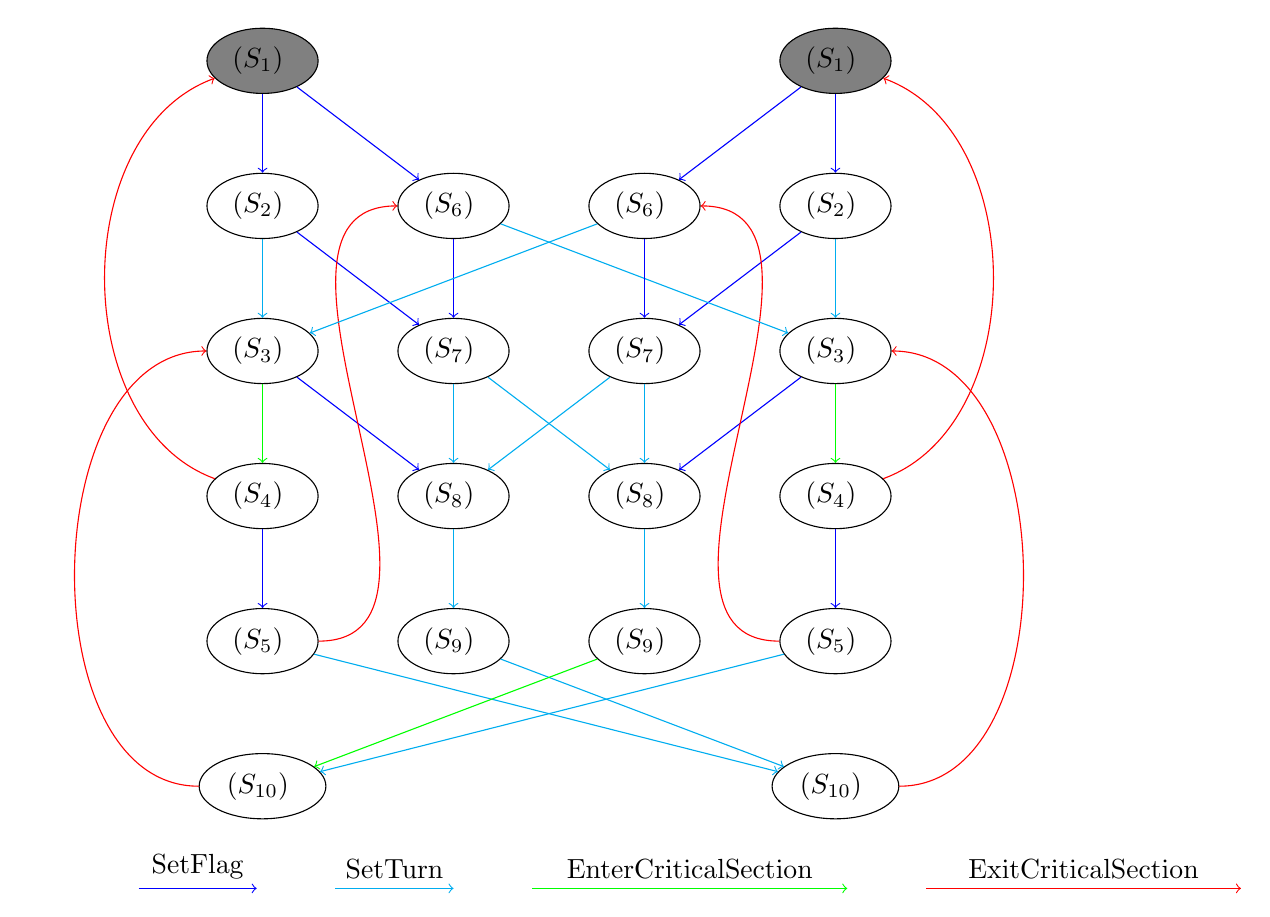
\begin{tikzpicture} [every text node part/.style={align=center}]
					
					\node[ellipse, draw, fill=gray] (s1) {\pa $(S_1)$ };
					\node[ellipse, draw] (s2) [below = of s1] {\pa $(S_2)$ };
					\node[ellipse, draw] (s3) [below = of s2] {\pa $(S_3)$ };
					\node[ellipse, draw] (s4) [below = of s3] {\pa $(S_4)$ };
					\node[ellipse, draw] (s5) [below = of s4] {\pa $(S_5)$ };
					
					\node[ellipse, draw] (s6) [right = of s2] {\pa $(S_6)$ };
					\node[ellipse, draw] (s7) [below = of s6] {\pa $(S_7)$ };
					\node[ellipse, draw] (s8) [below = of s7] {\pa $(S_8)$ };
					\node[ellipse, draw] (s9) [below = of s8] {\pa $(S_9)$ };
					
					
					\node[ellipse, draw] (q6) [right = of s6] {\pb $(S_6)$ };
					\node[ellipse, draw] (q7) [below = of q6] {\pb $(S_7)$ };
					\node[ellipse, draw] (q8) [below = of q7] {\pb $(S_8)$ };
					\node[ellipse, draw] (q9) [below = of q8] {\pb $(S_9)$ };
					
					
					\node[ellipse, draw] (q2) [right = of q6] {\pb $(S_2)$ };
					\node[ellipse, draw,fill=gray] (q1) [above= of q2]{\pb $(S_1)$ };
					\node[ellipse, draw] (q3) [below = of q2] {\pb $(S_3)$ };
					\node[ellipse, draw] (q4) [below = of q3] {\pb $(S_4)$ };
					\node[ellipse, draw] (q5) [below = of q4] {\pb $(S_5)$ };
					
					
					\node[ellipse, draw] (q10) [below = of s5] {\pb $(S_{10})$ };
					\node[ellipse, draw] (s10) [below = of q5] {\pa $(S_{10})$ };
					
					\coordinate[below left = of q10] (c1);
					\coordinate[right = 1.5cm of c1] (d1);
					\coordinate[right = 1cm of d1] (c2);
					\coordinate[right =1.5cm  of c2] (d2);
					\coordinate[right = of d2] (c3);
					\coordinate[right =4cm of c3] (d3);
					\coordinate[right = of d3] (c4);
					\coordinate[right = 4cm of c4] (d4);
					
					\draw [->,blue,text=black] (c1) to node[auto]{SetFlag} (d1);
					\draw [->,cyan,text=black] (c2) to node[auto]{SetTurn} (d2);
					\draw [->,green,text=black] (c3) to node[auto]{EnterCriticalSection} (d3);
					\draw [->,red,text=black] (c4) to node[auto]{ExitCriticalSection} (d4);
					
					\path[->]
					(s1) edge [blue] (s2)
					(s1) edge [blue] (s6)
					(q1) edge [blue] (q2)
					(q1) edge [blue] (q6)
					(s2) edge [cyan] (s3)
					(s2) edge [blue] (s7)
					(q2) edge [cyan] (q3)
					(q2) edge [blue] (q7)
					(s3) edge [green] (s4)
					(s3) edge [blue] (s8)
					(q3) edge [green] (q4)
					(q3) edge [blue] (q8)
					(s4) edge [blue] (s5)
					(q4) edge [blue] (q5)
					(s4) edge [red ,bend left=70] (s1)
					(q4) edge [red, bend right=70] (q1)
					(s5) edge [red,out=0,in=180] (s6)
					(s5) edge [cyan] (s10)
					(q5) edge [red,out=180,in=0] (q6)
					(q5) edge [cyan] (q10)
					
					(s6) edge [cyan] (q3)
					(s6) edge [blue] (s7)
					(q6) edge [cyan] (s3)
					(q6) edge [blue](q7)
					(s7) edge[cyan] (q8)
					(s7) edge[cyan] (s8)
					(q7) edge[cyan] (s8)
					(q7) edge[cyan] (q8)
					(s8) edge[cyan] (s9)
					(q8) edge [cyan](q9)
					(s9) edge [cyan](s10)
					(q9) edge[green] (q10)
					(s10) edge[out=0,in=0,red] (q3)
					(q10) edge[out=180,in=180,red] (s3)
					;
					
				\end{tikzpicture}
			
			\caption{State exploration diagram for Peterson's algorithm}
			\label{fig:petersonlockstatediagram}
			\end{figure}
		
				\begin{center}
					\begin{longtable}{ |c|p{10cm}| } 
						\hline
						\textbf{State Identifier} & \textbf{State Clause} \\
						\hline 
						\endhead
							\pa $(S_1)$  & $flag = (0 :> \FALSE  ;  1 :> \FALSE)$\newline
													$\AND state = (0 :> "Start"  ;  1 :> "Start")$\newline
													$\AND turn = 1$\\
							\hline
							\pa $(S_2)$   & $flag = (0 :> \TRUE  ;  1 :> \FALSE)$\newline
													$\AND state = (0 :> "RequestTurn"  ;  1 :> "Start")$\newline
													$\AND turn = 1$  \\ \hline
							\pa $(S_3)$   & $flag = (0 :> \TRUE  ;  1 :> \FALSE)$\newline
													$\AND state = (0 :> "Waiting"  ;  1 :> "Start")$\newline
													$\AND turn = 1$  \\ \hline
							\pa $(S_4)$   & $ flag = (0 :> \TRUE ; 1 :> \FALSE)$\newline
													$\AND state = (0 :> "CriticalSection" ; 1 :> "Start")$\newline
													$\AND turn = 1$  \\ \hline
							\pa $(S_5)$   & $ flag = (0 :> \TRUE ; 1 :> \TRUE)$\newline
													$\AND state = (0 :> "CriticalSection" ; 1 :> "RequestTurn")$\newline
													$\AND turn = 1$  \\ \hline
							\pa $(S_6)$   & $ flag = (0 :> \FALSE ; 1 :> \TRUE)$\newline
													$\AND state = (0 :> "Start" ; 1 :> "RequestTurn")$\newline
													$\AND turn = 1$  \\ \hline
							\pa $(S_7)$   & $\AND flag = (0 :> \TRUE ; 1 :> \TRUE)$\newline
													$\AND state = (0 :> "RequestTurn" ; 1 :> "RequestTurn")$\newline
													$\AND turn = 1$  \\ \hline
							\pa $(S_8)$   & $\AND flag = (0 :> \TRUE ; 1 :> \TRUE)$\newline
													$\AND state = (0 :> "Waiting" ; 1 :> "RequestTurn")$\newline
													$\AND turn = 1$  \\ \hline
							\pa $(S_9)$   & $\AND flag = (0 :> \TRUE ; 1 :> \TRUE)$\newline
													$\AND state = (0 :> "Waiting" ; 1 :> "Waiting")$\newline
													$\AND turn = 0$  \\ \hline
							\pa $(S_{10})$   & $\AND flag = (0 :> \TRUE ; 1 :> \TRUE)$\newline
													$\AND state = (0 :> "CriticalSection" ; 1 :> "Waiting")$\newline
													$\AND turn = 0$  \\ \hline
							\pb $(S_1)$  & $flag = (0 :> \FALSE  ;  1 :> \FALSE)$\newline
													$\AND state = (0 :> "Start"  ;  1 :> "Start")$\newline
													$\AND turn = 0$\\
							\hline
							\pb $(S_2)$   & $flag = (0 :> \FALSE  ;  1 :> \TRUE)$\newline
													$\AND state = (0 :> "Start"  ;  1 :> "RequestTurn")$\newline
													$\AND turn = 0$  \\ \hline
							\pb $(S_3)$   & $flag = (0 :> \FALSE  ;  1 :> \TRUE)$\newline
													$\AND state = (0 :> "Start"  ;  1 :> "Waiting")$\newline
													$\AND turn = 0$  \\ \hline
							\pb $(S_4)$   & $ flag = (0 :> \FALSE ; 1 :> \TRUE)$\newline
													$\AND state = (0 :> "Start" ; 1 :> "CriticalSection")$\newline
													$\AND turn = 0$  \\ \hline
							\pb $(S_5)$   & $ flag = (0 :> \TRUE ; 1 :> \TRUE)$\newline
													$\AND state = (0 :> "RequestTurn" ; 1 :> "CriticalSection")$\newline
													$\AND turn = 0$  \\ \hline
							\pb $(S_6)$   & $ flag = (0 :> \TRUE ; 1 :> \FALSE)$\newline
													$\AND state = (0 :> "RequestTurn" ; 1 :> "Start")$\newline
													$\AND turn = 0$  \\ \hline
							\pb $(S_7)$   & $\AND flag = (0 :> \TRUE ; 1 :> \TRUE)$\newline
													$\AND state = (0 :> "RequestTurn" ; 1 :> "RequestTurn")$\newline
													$\AND turn = 0$  \\ \hline
							\pb $(S_8)$   & $\AND flag = (0 :> \TRUE ; 1 :> \TRUE)$\newline
													$\AND state = (0 :> "RequestTurn" ; 1 :> "Waiting")$\newline
													$\AND turn = 0$  \\ \hline
							\pb $(S_9)$   & $\AND flag = (0 :> \TRUE ; 1 :> \TRUE)$\newline
													$\AND state = (0 :> "Waiting" ; 1 :> "Waiting")$\newline
													$\AND turn = 1$  \\ \hline
							\pb $(S_{10})$   & $\AND flag = (0 :> \TRUE ; 1 :> \TRUE)$\newline
													$\AND state = (0 :> "Waiting" ; 1 :> "CriticalSection")$\newline
													$\AND turn = 1$  \\ \hline
							
						\hline
						\caption{State legend for the state exploration diagram in Figure \ref{fig:petersonlockstatediagram}}
					\end{longtable}
				\end{center}
			
			
			
		\newpage
			\section*{Appendix C}
			\label{codebase}
			\subsection*{\tla specification for Peterson's algorithm.} \label{petersonspec}
			\ruleline{MODULE \textit{peterson\_lock} }
			$\EXTENDS Integers, TLAPS$\\\\
			$\VARIABLES turn, state, flag$\\\\
			$vars \triangleq  \langle turn, state, flag \rangle$\\\\
			$ProcSet \triangleq \{0,1\} $\\\\
			$States \triangleq \{"Start", "RequestTurn", "Waiting", "CriticalSection"\} $\\\\
			$Not(i) \triangleq 1-i $\\\\
			$ Init \triangleq flag = [i \in ProcSet \mapsto \FALSE]$ \\
			\hspace*{0.8cm}$\AND Turn \in \{0,1\}$\\
			\hspace*{0.8cm}$\AND  Start =  [i \in ProcSet \mapsto "Start"]$\\\\
			$ SetFlag(p) \triangleq state[p] = "Start"$ \\
			\hspace*{0.8cm}$\AND flag' = [flag \EXCEPT ![p] = \TRUE]$\\
			\hspace*{0.8cm}$\AND  state' = [state \EXCEPT ![p] = "RequestTurn"]$\\
			\hspace*{0.8cm}$\AND \UNCHANGED \langle turn \rangle $\\\\
			$ SetTurn(p) \triangleq state[p] = "RequestTurn"$ \\
			\hspace*{0.8cm}$\AND turn' = Not(p)$\\
			\hspace*{0.8cm}$\AND  state' = [state \EXCEPT ![p] = "Waiting"]$\\
			\hspace*{0.8cm}$\AND \UNCHANGED \langle flag \rangle $\\\\
			$ EnterCriticalSection(p) \triangleq state[p] = "Waiting"$ \\
			\hspace*{0.8cm}$\AND (flag[Not(p)] = \FALSE \OR turn = p)$\\
			\hspace*{0.8cm}$\AND  state' = [state \EXCEPT ![p] = "CriticalSection"]$\\
			\hspace*{0.8cm}$\AND \UNCHANGED \langle turn, flag \rangle $\\\\
			$ ExitCriticalSection(p) \triangleq state[p] = "CriticalSection""$ \\
			\hspace*{0.8cm}$\AND  flag' = [flag \EXCEPT ![p] = \FALSE]$\\
			\hspace*{0.8cm}$\AND  state' = [state \EXCEPT ![p] = "Start"]$\\
			\hspace*{0.8cm}$\AND \UNCHANGED \langle turn \rangle $\\\\
			$Next \triangleq \exists p \in ProcSet:$\\
			\hspace*{0.8cm}$ \OR setFlag(p)$\\
			\hspace*{0.8cm}$ \OR SetTurn(p)$\\
			\hspace*{0.8cm}$ \OR EnterCriticalSection(p)$\\
			\hspace*{0.8cm}$ \OR ExitCriticalSection(p)$\\\\
			$Spec \triangleq Init \AND \square [Next]_{vars}$\\\\
			$proc(self) \triangleq$\\
			\hspace*{0.8cm}$ \OR setFlag(self)$\\
			\hspace*{0.8cm}$ \OR SetTurn(self)$\\
			\hspace*{0.8cm}$ \OR EnterCriticalSection(self)$\\
			\hspace*{0.8cm}$ \OR ExitCriticalSection(self)$\\\\
			$ ExecutionInvariant \triangleq \forall i \in ProcSet:"$ \\
			\hspace*{0.8cm}$state[i] \in States \setminus  \{"Start"\} \implies flag[i] $\\
			\hspace*{0.8cm}$\AND  state[i] \in \{"CriticalSection"\} \implies state[Not(i)] \notin \{"CriticalSection"\}$\\
			\hspace*{0.8cm}$\AND state[Not(i)] \in \{"Waiting"\} \implies turn = i$\\\\
			$ TypeInvariant \triangleq state \in [ProcSet \rightarrow States]$ \\
			\hspace*{0.8cm}$\AND turn \in ProcSet$\\
			\hspace*{0.8cm}$\AND flag \in [ProcSet \rightarrow \{true, false\}]$\\\\
			$MutualExclusion \triangleq \lnot(state[0] = "CriticalSection" \AND state[1] = "CriticalSection")$\\\\
			$Inv \triangleq ExecutionInvariant \AND TypeInvariant$\\
			
			\hrule
			
			\subsection*{\tla proof specification for mutual exclusion}
			\ruleline{MODULE \textit{peterson\_lock} }
			...\tla spec for peterson's lock \ref{petersonspec}...\\\\
			$\THEOREM Spec \implies \square MutualExclusion$\\
			$\PROOF$\\
			\hspace*{0.8cm}$\langle1\rangle1. Init \implies Inv$\\
			\hspace*{1.2cm} $\BY \DEFS Init, Inv, TypeInvariant, ExecutionInvariant, vars,States,ProcSet$\\\\
			\hspace*{0.8cm}$\langle1\rangle2. Inv \AND [Next]_{vars} \implies Inv'$\\
			\hspace*{1.2cm} $\BY \DEFS Init, Inv, TypeInvariant, ExecutionInvariant, vars,States,ProcSet$\\\\
			\hspace*{1.6cm}$\langle2\rangle1. \SUFFICES \ASSUME Inv,Next\  \PROVE Inv'$\\
			\hspace*{2cm} $\BY \DEFS ExecutionInvariant,TypeInvariant,Inv,vars$\\\\
			\hspace*{1.6cm}$\langle2\rangle2. TypeInvariant'$\\
			\hspace*{2cm} $\BY \langle2\rangle1$\\
			\hspace*{2cm}$ \DEFS Inv, TypeInvariant, Next, proc, Not, States, ProcSet,$\\
			\hspace*{2cm}$ SetFlag, SetTurn, EnterCriticalSection, ExitCriticalSection$\\\\
			\hspace*{1.6cm}$\langle2\rangle3. ExecutionInvariant'$\\
			\hspace*{2.8cm}$\langle3\rangle1. \SUFFICES \ASSUME \NEW j \in ProcSet \PROVE ExecutionInvariant!(j)'$\\
			\hspace*{3.2cm}$\BY \DEFS ExecutionInvariant,ProcSet$\\\\
			\hspace*{2.8cm}$\langle3\rangle2. \PICK i \in ProcSet : proc(i) $\\
			\hspace*{3.2cm}$\BY \langle2\rangle1 \DEFS Next,ProcSet,proc, SetFlag, SetTurn,$\\
			\hspace*{3.2cm}$EnterCriticalSection, ExitCriticalSection$\\\\
			\hspace*{2.8cm}$\langle3\rangle3. \CASE i =j $\\
			\hspace*{3.2cm}$\BY \langle2\rangle1 , \langle3\rangle2\  \DEFS ExecutionInvariant, TypeInvariant, Inv, proc,$\\
			\hspace*{3.2cm}$Not,ProcSet, SetFlag, SetTurn, EnterCriticalSection, ExitCriticalSection$\\\\
			\hspace*{2.8cm}$\langle3\rangle3. \CASE i \neq j $\\
			\hspace*{3.2cm}$\BY \langle2\rangle1 , \langle3\rangle2\  \DEFS ExecutionInvariant, TypeInvariant, Inv, proc, Not,ProcSet,$\\
			\hspace*{3.2cm}$SetFlag, SetTurn, EnterCriticalSection, ExitCriticalSection$\\\\
			\hspace*{2.8cm}$\langle3\rangle. \QED \BY \langle3\rangle3 , \langle3\rangle4 $\\\\
			\hspace*{1.6cm}$\langle2\rangle4. \QED \BY \langle2\rangle2 , \langle2\rangle3 \DEF Inv $\\\\
			\hspace*{0.8cm}$\langle1\rangle3. Inv \implies MutualExclusion$\\
			\hspace*{1.2cm}$ \BY\DEFS Inv, MutualExclusion,ProcSet,Not,ExecutionInvariant,TypeInvariant$\\\\
			\hspace*{0.8cm}$\langle1\rangle4. \QED \BY \langle1\rangle1,\langle1\rangle2,\langle1\rangle3,\langle1\rangle4, \PTL$\\
			\hspace*{1.2cm}$\DEFS MutualExclusion,Spec,ExecutionInvariant, TypeInvariant, Inv, $\\
			\hspace*{1.2cm} $proc, Not,ProcSet, SetFlag, SetTurn, EnterCriticalSection, ExitCriticalSection$\\
			
			\hrule
			
			
			%%%%%%%%%%%%%%%%%%%%%%%%%%%%%%%%%%%%%%%%%%%%%%%%%%%%%%%%%%%%%%%%%%%%%%%%%%%%%%%
			\newpage
			\nocite{*}
			\bibliographystyle{eptcs}
			\bibliography{references}
			
			%%%%%%%%%%%%%%%%%%%%%%%%%%%%%%%%%%%%%%%%%%%%%%%%%%%%%%%%%%%%%%%%%%%%%%%%%%%%%%%
		\end{document}
		%%%%%%%%%%%%%%%%%%%%%%%%%%%%%%%%%%%%%%%%%%%%%%%%%%%%%%%%%%%%%%%%%%%%%%%%%%%%%%%
